\documentclass[11pt,a4paper]{scrartcl}
\usepackage[czech]{babel}
\usepackage[utf8]{inputenc}
\usepackage{graphicx}
\usepackage{float}

\begin{document}
	\title{Semestrální práce z předmětu KIV/PPR}
	\subtitle{Prolomení šifry SkipJack}
	\author{Zdeněk Valeš}
	\date{22.11. 2018}
	\maketitle
	\newpage
	
	\section{Zadání}
	Vaším úkolem bude prolomit šifru SkipJack. Tuto šifru je výpočetně náročné prolomit hrubou silou, nicméně lze zkusit i sofistikovanější metody např. genetické a evoluční algoritmy. Abyste prolomení urychlili, lze referenční kód přepsat a vektorizovat na úrovni instrukcí, pomocí GPU, případně ho distribuovat pomocí MPI.
	
	Samostatná práce využije alespoň dvě z celkem tří možných technologií:
	
	\begin{itemize}
		\item Paralelní program pro systém se sdílenou pamětí - C++, popř. WinAPI
		\item Program využívající asymetrický multiprocesor - konkrétně x86 CPU a OpenCL kompatibilní GPGPU - C++ AMP
		\item Paralelní program pro systém s distribuovanou pamětí - C++ MPI
	\end{itemize}

	Práci implementujte v jazyce C++ do základu aplikace, který je k dispozici na CourseWare.
	
	\section{Popis řešení}
	Vstupem prolamovací funkce je zašifrovaný blok a referenční blok. Cílem algoritmu je nalezení klíče (jedince) po jehož použití v dešifrovací funkci bude vstupní blok identický s referenčním. Algoritmus je znázorněn na obrázku \ref{fig:alg}.
	
	K prolomení šifry jsem použil diferenciální evoluci s Hammingovou vzdáleností jako cenovou funkcí. Části programu jsou paralelizované pomocí kníhoven Intel TBB a OpenCL.
	
	\begin{figure}[!h]
		\centering
		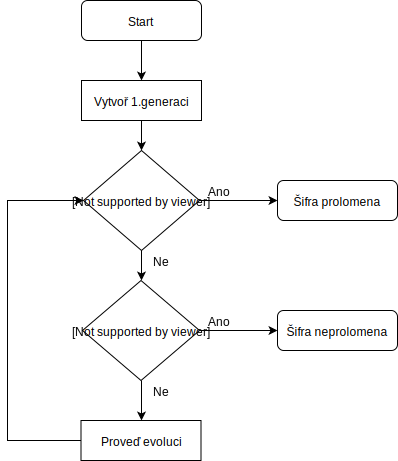
\includegraphics[height=7.5cm]{img/alg-flowchart}
		\caption{Algoritmus řešení}
		\label{fig:alg}
	\end{figure}
	
	\subsection{Diferenciální evoluce}
	Diferenciální evoluce je v principu velmi podobná klasickým genetickým algoritmům. Liší se od nich počtem rodičů (\textgreater2) potřebným k tvorbě potomka a pořadím operací mutace, křížení \cite{hlavacek_de}. 
	
	Při evoluci jedince se nejprve mutací získá šumový vektor, který se pak zkříží s aktivním jedincem. Pokud má takto vzniklý jedinec lepší skóre než aktivní, použije se do nové populace.
	Evoluce je řízena dvěma parametry: mutační konstantou \textit{F} a prahem křížení \textit{CR}. Doporučené hodnoty jsou 0,3 -- 0,9 pro \textit{F} a 0,8 -- 0,9 pro \textit{CR} \cite{hlavacek_de}. V mém řešení jsem zvolil hodnoty $F=0,3$ a $CR=0,5$.
	
	\subsubsection{Cenová funkce}
	Jako cenovou funkci jsem použil variantu Hammingovo vzdálenosti dešifrovaného bloku od bloku referečního. Během implementace jsem experimentoval s více cenovými funkcemi a držel jsem se konvence větší skóre znamená lepšího jedince. U Hammingovo vzdálenosti to ale neplatí, proto jsem tuto vzdálenost odečetl od maximální možné vzdálenosti (viz rovnice \ref{eq:fitness}).
	
	\begin{equation}
		fitness = D_{max} - D(decrypted,reference)
		\label{eq:fitness}
	\end{equation}
	
	Vzhledem k povaze šifry SkipJack není tato cenová příliš vhodná, jak je vidět na obrázku \ref{fig:fitness-chart}. Během přednášek nám byla vyučujícím doporučena dvojrozměrná cenová funkce, tu se mi bohužel nepodařilo funkčně naimplementovat.
	
	\begin{figure}[!h]
		\centering
		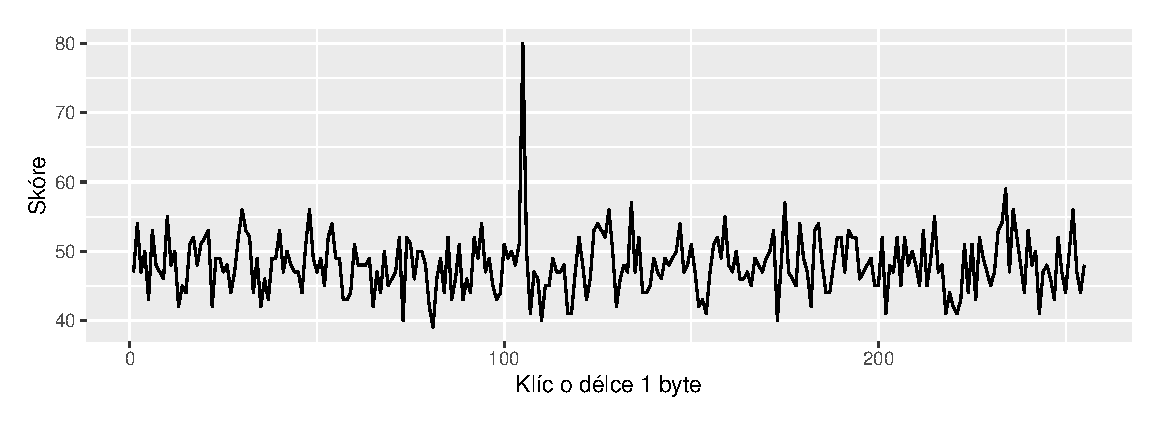
\includegraphics[width=15cm]{img/fitness-plot}
		\caption{Hodnoty fitness funkce pro klíč délky 1}
		\label{fig:fitness-chart}
	\end{figure}

	Kromě Hammingovo vzdálenosti dešifrovaného bloku od referenčního jsem experimentoval i se vzdáleností jedince od referenčního hesla. V tomto případě algoritmus konverguje dobře (100-200 generací), nicméně znalost hesla není běžný případ a proto jsem tuto cenovou funkci použil pouze k odstranění chyb evolučního algoritmu.
	\subsection{Paralelizace}
	Vektory na mutaci ne-e. Použito TBB + OpenCL, popis paralelizace evoluce (parallel\_for)
	
	\section{Výsledky}
	
	\section{Závěr}
	
	\begin{thebibliography}{9}
		\bibitem{hlavacek_de}
		HLAVÁČEK, Jiří. \textit{Moderní adaptivní diferenciální evoluce} [online]. Zlín, 2015 [cit. 2018-11-22]. Dostupné z: \textless https://theses.cz/id/vs0ow2/\textgreater. Diplomová práce. Univerzita Tomáše Bati ve Zlíně, Fakulta aplikované informatiky. Vedoucí práce doc. Ing. Roman Šenkeřík, Ph.D
	\end{thebibliography}
	
\end{document}
